\chapter{Materials \& Methods}

% 학위 논문의 결과를 도출하는 데에 사용한 실험 재료와 방법을 타인이 반복 실험 시 동일한 결과를 얻을 수 있을 정도로 자세히 기술한다. 방법에 따라 다음과 같이 부제를 넣어 기술한다.

% 예)
% 2.1 식물 재료 및 생장 조건
% 2.2 뿌리 관속 조직 관찰
% 2.3 유전자 발현 분석

\section{Space Optimization}

\subsection{Diff-index Compression}

As is described in chapter 2, the diff-index created in the k-mer extraction step will store multiple \texttt{USHRT\_MAX} as long as the difference is larger than \texttt{USHRT\_MAX}. This will make any k-mer difference larger than $4 \times \mathtt{USHRT\_MAX} = 262140$ require a larger space to store than the original \texttt{unsigned long representation}. This situation is not uncommon especially when $k$ is large.
\autoref{fig:k11_space} showed the space consumption of the diff-index created in the k-mer extraction step when $k = 11$. Without optimization, the diff-index (k-mer table) and its corresponding ID table will take up 17 GB of space for a merely 1GB-sized database. Such huge space consumption is undesirable and need to be optimized.



\section{Speed Optimization}

\subsection{}

\section{Sensitivity Improvement}


\begin{figpage}
\begin{figure}[t]
\centering
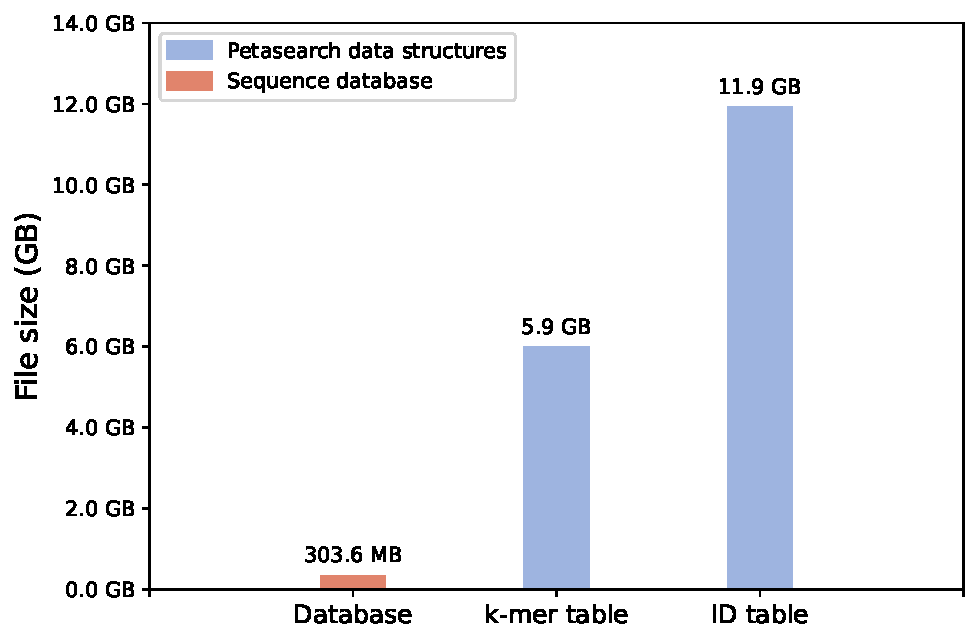
\includegraphics[width=0.8\textwidth]{images/k11_space_consumption.pdf}
\caption{Visualizaiton of k-mer table and ID table sizes when $k = 11$. The database is the \texttt{UniProtKB/Swiss-Prot} database obtained through \texttt{mmseqs databases UniProtKB/Swiss-Prot swissprot tmp} command. Without optimization, the sizes of \texttt{petasearch} data structures are 6.46 times and 12.92 times larger than the sequence database.}
\label{fig:k11_space}
\end{figure}
\end{figpage}
